%! TEX root = uts_gbrteknik_temu8.tex
% the main TeX file which is intended to compile, :VimtexReload after adjustment
% :h vimtex-tex-root
\documentclass[../gbr_teknik.tex]{subfiles}
% \includeonlyframes{current}
% \setbeameroption{hide notes} % Only slides
% \setbeameroption{show only notes} % Only notes
% \setbeameroption{show notes on second screen=right} % Both

\begin{document}

\begin{frame}[t,mycolor=digiPH_white,mytitle=standard,light]
	\txt{digiPH_gray}{digiPH_darkblue}{
		Buatlah gambar pandangan atas dan potongan dari depan untuk benda ``Dudukan Penutup" di bawah ini pada kertas A4, cantumkan tanda pengerjaan dan toleransi lubangnya. Pandangan depan sesuai tanda anak panah}

\end{frame}

\begin{frame}[mytitle=standard,t,mycolor=digiPH_gray,light]
	\begin{figure}
		\begin{center}
			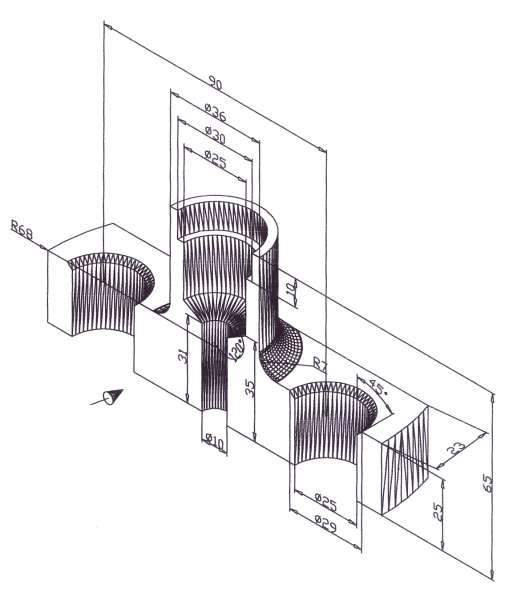
\includegraphics[height=.88\textheight]{../figures/uts_gbr_teknik.jpeg}
			% filename may not contain space but _
		\end{center}
		\caption{Ujian Tengah Semester}
	\end{figure}

\end{frame}

\end{document}
